
\documentclass{article}
\usepackage{amsmath}
\usepackage[margin=1in]{geometry}
\usepackage{amsfonts}
\usepackage{hyperref}
\usepackage{graphicx}
\usepackage{siunitx}
\usepackage{cancel}
\usepackage{xfrac}


\begin{document}
	
	\title{Curl}
	\author{Andy Chong Sam}
	\date{}
	\maketitle
	
	
	\section{Overview}
	
	\par \noindent The curl operator describes the rotation tendency of a vector field. Both its input and output are vectors. In the cases when we consider only two dimensions, the result of curl is a scalar.
	\newline
	\par \noindent If a vector field is defined by \(F = <P,Q>\) then its two dimdensional curl is defined as:
	
	\begin{flalign}
		\nabla \times F = \frac{\partial Q}{\partial x} - \frac{\partial P}{\partial y}
	\end{flalign}

	\par\noindent If \(F=<P,Q,R>\) we can calculate a three dimensional curl with:
	
	\begin{flalign}
		\nabla \times F = (\frac{\partial R}{\partial y} - \frac{\partial Q}{\partial z}) \vec i\;\; +\;\; (\frac{\partial P}{\partial z} - \frac{\partial R}{\partial x})\vec j \;\; + (\frac{\partial Q}{\partial x} - \frac{\partial P}{\partial y})\vec k
	\end{flalign}

	\par\noindent From Expressions (1) and (2) we again note that the latter produces a vector, and that its third component is just the two dimensional curl. 

	\section{Geometric Intuition}
	
	\par\noindent To start we will note that the orthodox direction of rotation is counter clockwise. Fields that induce a counter clockwise rotation will have a positive curl. We can start out by imagining a particle on the \(xy\) plane. 
	\newline
	
				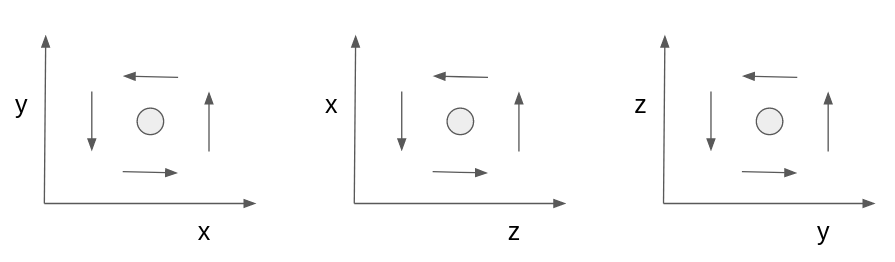
\includegraphics[width=15cm]{curl.png}
					\begin{center}
					Figure 1
				\end{center}
				
			\par \noindent In Figure 1's left graph, we've generalized what happens to a particle when a field induces positive curl. In these diagrams the arrows represent the field. We note that as \(x\) increases, the \(Q\) component of the field has a tendency to shift from negative to positive. Likewise as as \(y\) increases, the \(P\) component becomes more negative. In order to guarantee a positive value if the field is inducing a counter clockwise rotation we can  take the change of \(R\) with respect to \(y\) (which will be positive) and subtract from it the change of \(P\) with respect to \(y\) which will be negative. From this intuition, we get \(\frac{\partial Q}{\partial x} - \frac{\partial P}{\partial y}\) as the two dimensional curl.
			\newline
			\par\noindent In our analysis so far we've imagined that the field can only induce rotation on the \(xy\) plane. Because \(z\) is fixed in this scenario, the two dimensional curl is the \(\vec k\) component of the three dimensional curl. We can think of this as the observed rotation viewed from \(z\)'s perspective.
			\newline
			\par\noindent Looking again at Figure 1, the central diagram describes a hypothetical counter clockwise rotation from the perspective of \(y\). As \(z\) increases, the \(P\) component of the field becomes more positive and as \(x\) increases, the \(R\) compoment becomes more negative. So to guarantee a positive value we can write \(\frac{\partial P}{\partial z} - \frac{\partial R}{\partial x}\). The same analysis can be performed with Figure 1's right graph.
			

\section{Examples}
	\framebox{
		\parbox{\linewidth}{
			
			\textbf{Ex. 1} Calculate \(\nabla \times F\) given \(F(x,y,z) = \frac{1}{\sqrt{x^2+y^2+z^2}}(x\; \vec i + y\; \vec j + z\; \vec k)\)
			\newline
			\par\noindent Source:
			\newline
			\begin{flalign*}
				\frac{\partial R}{\partial y} =  \frac{zy}{2\sqrt{x^2+y^2+z^2}} \;\;\;
				\frac{\partial Q}{\partial z} =  \frac{zy}{2\sqrt{x^2+y^2+z^2}} \;\;\;
				\frac{\partial P}{\partial z} =  \frac{xz}{2\sqrt{x^2+y^2+z^2}} \\
				\frac{\partial R}{\partial x} =  \frac{xz}{2\sqrt{x^2+y^2+z^2}} \;\;\;
				\frac{\partial Q}{\partial x} =  \frac{xy}{2\sqrt{x^2+y^2+z^2}} \;\;\;
				\frac{\partial P}{\partial y} =  \frac{xy}{2\sqrt{x^2+y^2+z^2}}
			\end{flalign*}
		
			\begin{flalign*}
	\nabla \times F = (\frac{\partial R}{\partial y} - \frac{\partial Q}{\partial z}) \vec i\;\; +\;\; (\frac{\partial P}{\partial z} - \frac{\partial R}{\partial x})\vec j \;\; + (\frac{\partial Q}{\partial x} - \frac{\partial P}{\partial y})\vec k
			\end{flalign*}
		
			\begin{flalign*}
							\nabla \times F = 0\;\vec i + 0\;\vec j + 0\;\vec k
			\end{flalign*}
		
			\begin{center}
			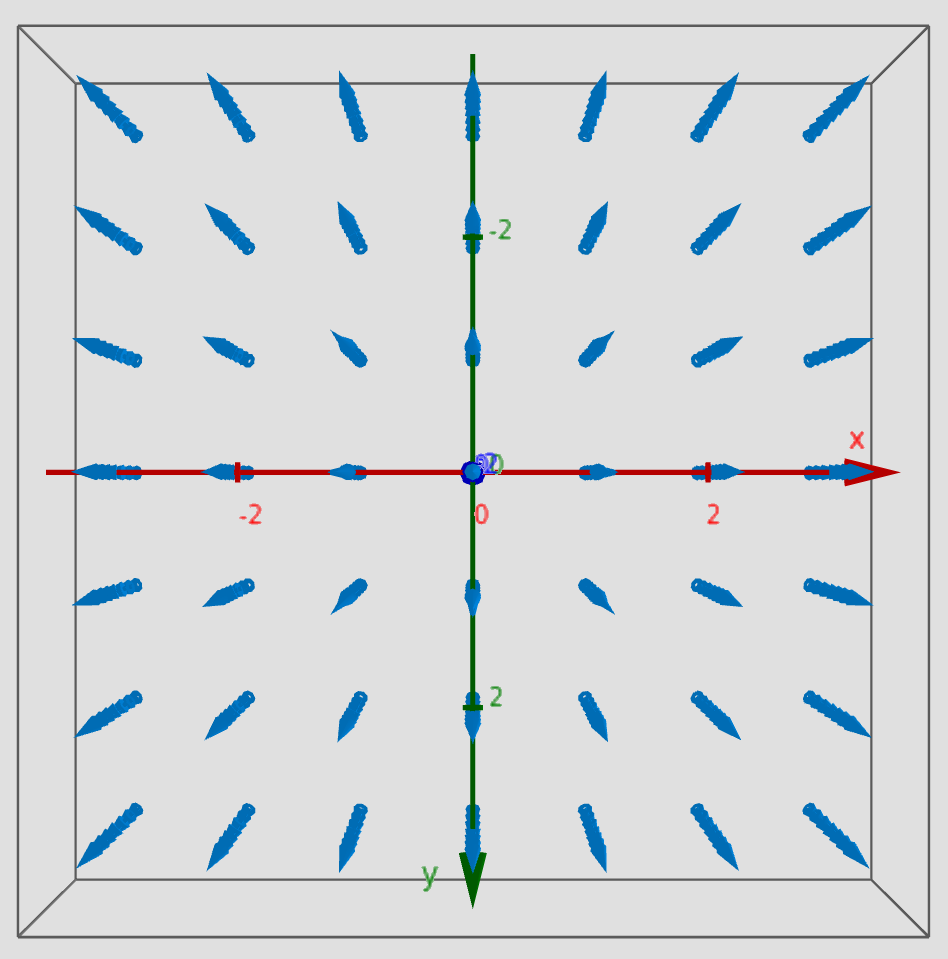
\includegraphics[width=7cm]{ex1field.png}
			\end{center}
			\begin{center}
				Figure 2
			\end{center}
		
		\par\noindent No curl is present. A graph of the field (top down) is shown in Figure 2. We can intuitively see that this field is incapable of inducing rotation.

		
	}
}
\newpage
	\framebox{
	\parbox{\linewidth}{
		
		\textbf{Ex. 2} Calculate \(\nabla \times F\) where \(F=xye^z\;\vec i + yze^x\;\vec k\)
		\newline
		
				\par\noindent Source:
				
			\begin{flalign*}
	\frac{\partial R}{\partial y} =  ze^x \;\;\;
	\frac{\partial Q}{\partial z} =  0 \;\;\;
	\frac{\partial P}{\partial z} =  xye^z \\
	\frac{\partial R}{\partial x} =  yze^x \;\;\;
	\frac{\partial Q}{\partial x} =  0 \;\;\;
	\frac{\partial P}{\partial y} =  xe^z
\end{flalign*}		
		
					\begin{flalign*}
			\nabla \times F = (\frac{\partial R}{\partial y} - \frac{\partial Q}{\partial z}) \vec i\;\; +\;\; (\frac{\partial P}{\partial z} - \frac{\partial R}{\partial x})\vec j \;\; + (\frac{\partial Q}{\partial x} - \frac{\partial P}{\partial y})\vec k
		\end{flalign*}
		
		\begin{flalign*}
			\nabla \times F = ze^x\;\vec i + xye^z - yze^x\;\vec j -xe^z\;\vec k
		\end{flalign*}
}}
\end{document}